\documentclass[conference]{IEEEtran}

\usepackage[utf8]{inputenc}
\usepackage{cite}
\usepackage{amsmath}
\usepackage{graphicx}
\usepackage[english,hungarian]{babel}
\usepackage[section]{placeins}
\usepackage{subfigure}
\usepackage{float}
    
\begin{document}
\selectlanguage{english}

\title{Image Inpainting for Regular Holes Using Partial Convolutions\\
	{\large \textbf{Szabályos lyukak digitális retusálása részleges konvolúcióval}}\\
	{\large \textit{Team:} DeepPurple}\\
}

\author{
	\IEEEauthorblockN{Dávid Kékesi}
	\IEEEauthorblockA{
		J9PCWO \\
		david.kekesi@gmail.com}
\and
	\IEEEauthorblockN{Mátyás Sándor}
	\IEEEauthorblockA{
		YHMJTY\\
		sandor.matya@t-online.hu}
\and
	\IEEEauthorblockN{Zoltán Király}
	\IEEEauthorblockA{
		G24TCR\\
		ze.kiraly@gmail.com}
}

\maketitle

\selectlanguage{english}
\begin{abstract}\\
Image inpainting is the process of restorating a missing, undesired or damaged part of an image.
Initially, the technical faults of early cameras (scratches, stains) were corrected by experts while the development of photos. 
Although nowadays the manipulation of images happens digitally, the proper way of inpainting still requires skilled hands.
Many effort have been made to solve the automatization of this method. In this paper, we represent our work on applying
a model based on partial convolutions to fill missing parts of images with natural looking content.
\end{abstract}

\selectlanguage{hungarian}
\begin{abstract}\\
A folyamatot, melynek során egy kép sérült, nem kívánatos vagy hiányzó részeit eltüntetjük, retusálásnak nevezzük.
A fényképezőgépek technikai hibáit (karcok, pöttyök) eleinte manuálisan küszöbölték ki a szakemberek a fotók előhívás során.
Bár a fényképek manipulációja napjainkban digitális úton történik, a megfelelő retusálás továbbra is hozzáértő kezeket igényel.
A művelet automatizálására számos megoldás létezik, Jelen munkában azt mutatjuk be, hogy hogyan alkalmaztunk egy
részleges konvolúcióra épülő modellt, mely képes képek hiányzó részeit kiegészíteni természetes hatású tartalommal.
\end{abstract}

\selectlanguage{english}
\begin{IEEEkeywords}
Deep Learning, Image inpainting, GAN
\end{IEEEkeywords}

\section{Introduction}
At the initial stage of the project the team had consensus that we would like to work on a project involved in image processing. In the field of image inpainting Nvidia’s 2018 solution based on partial convolutions was a huge step forward, so this field seemed to be exciting enough to start working on. All of the team members are perfectly new to the field of deep learning, so we had to start with lots of reading and information gathering. Fundamentally it seemed that there are two widely used approahches for restoring the missing parts of an image. The first one is using a GAN, where a VAE based generator network, and a discriminator network, competing each other, creates more and more realistic images in a given domain. With a bit of modification this approach can be used not only for generating images from scratch, but for filling in the missing parts of an image as well. The other approach was based on the paper of Liu \cite{nvidia_paper}. It was obvious that both approaches require a lot of time spent on training, and we had limited hardware resources. The GAN approach had a further drawback: it’s very hard to do it in a way that it really gives usable results, and the network needs a lot of fine tuning. Reading the above linked paper, we found out that implementing the partial convolution can lead us to a shortcut, where we can use transfer learning by reusing the alredy trained VGG\_16 network, saving us a reasonable amount of GPU time. Even so the adaptation of the paper was quite difficult for us, being total beginners, so our final solution relies heavily on a Keras adaptation that we found on GitHub \cite{pconv_keras}. Even with the use of transfer learning we had to train the adapted model for 7-8 hours per training (60-70 epochs) on a GTX 1060, but the final results are quite impressive on the chosen dataset

\section{Initial method}
There are two main components of the learning process in the chosen problem: an encoder an a discriminator network has to work against each other, in order tomotivate eachother to produce better and better outputs, thus eliminating the differences between the original and generated pictures, and on the discriminator side to learn the  smaller and smaller differences between the generated and real pictures, thus motivating the encoder to eliminate the said smaller and smaller differences as well. 

\begin{figure}[H]
  \centering
  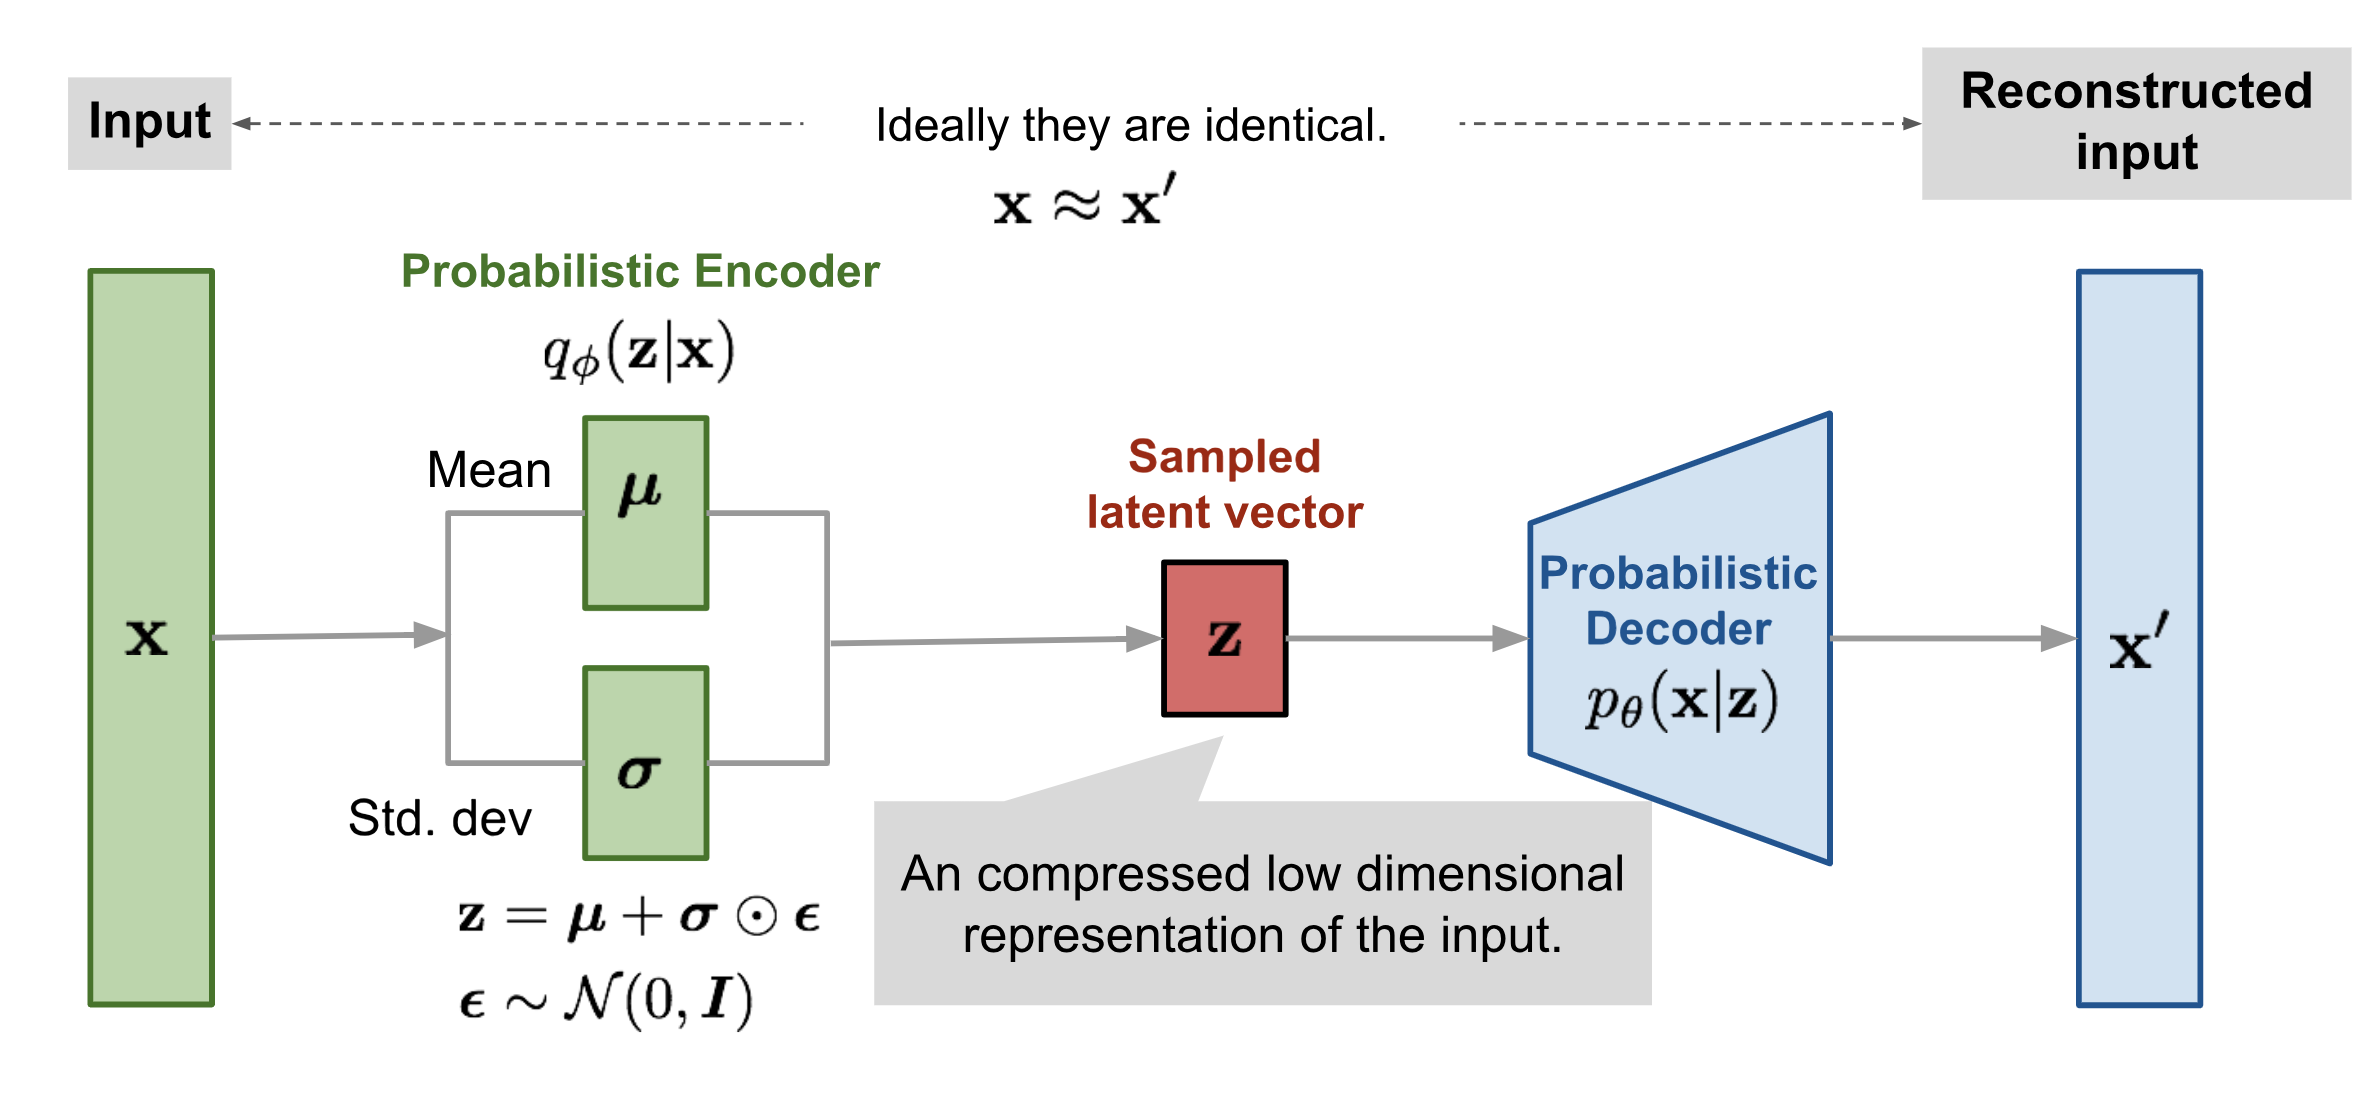
\includegraphics[width=80mm, keepaspectratio]{figures/vae-gaussian.png}
\end{figure}

\begin{figure}[H]
  \centering
  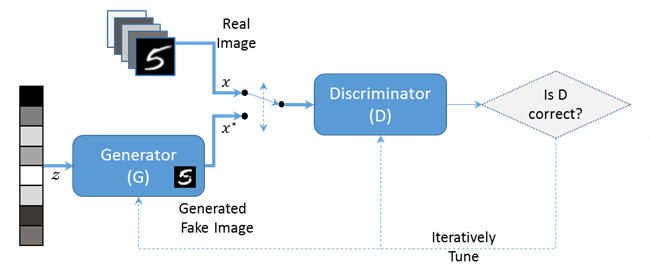
\includegraphics[width=80mm, keepaspectratio]{figures/GAN_basic_flow.png}
\end{figure}

We tried to use the above described method to solve the given problem, but before implementing the intially found method as a solution, we found a more modern approach, one that was more promising, and indeed proved to be a viable and fruitful solution.

\section{System design}
\subsection{Partial convolution}
The applied network relies on the use of a layer consisting of partial convolution and automatic mask update.
The partial convolution can be defined as
\begin{equation}
{x}' = \begin{cases}
W^T(X \odot M) \frac{sum(1)}{sum(M)} + b, & \text{if } sum(M) > 0 \\
0, & \text{otherwise}
\end{cases}
\end{equation}
for every location, where W is the weight matrix for the convolution filter and b is its corresponding bias. X are the feature values for the current convolution window and M is the curresponding binary mask.
$\odot$ denotes element-wise multiplication, and 1 has the same shape as M but with all elements being 1. Output values depend only on the unmasked inputs. The scaling factor sum(1)/sum(M) applies appropriate scaling for the varying amount of valid (unmasked) inputs.

After each partial convolution operation, we then update our mask as follows:
if the convolution was able to condition its output on at least one valid input value, then we mark that location as valid. This is expressed as:

\begin{equation}
{m}' = \begin{cases}
1, & \text{if } sum(M) > 0 \\
0, & \text{otherwise}
\end{cases}
\end{equation}

And can be implemented in any deep learning framewrok as part of the forward pass. With sufficient successive applications of the partial convolution layer, any mask will eventually be all ones, if the input contained any valid pixels.

\subsection{Partial Convolution as Padding}
We use the partial convolution with
appropriate masking at image boundaries. This ensures
that the inpainted content at the image border will not be affected by invalid values outside of the image – which can be interpreted as another hole.

\subsection{Model}
\begin{table}[H]
    \centering
    \scalebox{0.73}{
    \begin{tabular}{c|c|c|c|c|c}
        Module Name& Filter Size & \# Filters/Channels & Stride/Up Factor & BatchNorm & Nonlinearity\\
        \hline
         PConv1& 7$\times$7& 64& 2& -& ReLU\\
         PConv2& 5$\times$5& 128& 2& Y& ReLU\\
         PConv3& 5$\times$5& 256& 2& Y& ReLU\\
         PConv4& 3$\times$3& 512& 2& Y& ReLU\\
         PConv5& 3$\times$3& 512& 2& Y& ReLU\\
         PConv6& 3$\times$3& 512& 2& Y& ReLU\\
         PConv7& 3$\times$3& 512& 2& Y& ReLU\\
         PConv8& 3$\times$3& 512& 2& Y& ReLU\\
         \hline
         NearestUpSample1& & 512& 2 & - & -\\
         Concat1(w/ PConv7)& &512+512&  & - & -\\
         PConv9&3$\times$3& 512 &1& Y& LeakyReLU(0.2)\\
         \hline
         NearestUpSample2& & 512& 2 & - & -\\
         Concat2(w/ PConv6)& &512+512&  & - & -\\
         PConv10&3$\times$3& 512 &1& Y& LeakyReLU(0.2)\\
         \hline
         NearestUpSample3& & 512& 2 & - & -\\
         Concat3(w/ PConv5)& &512+512&  & - & -\\
         PConv11&3$\times$3& 512 &1& Y& LeakyReLU(0.2)\\
         \hline
         NearestUpSample4& & 512& 2 & - & -\\
         Concat4(w/ PConv4)& &512+512&  & - & -\\
         PConv12&3$\times$3& 512 &1& Y& LeakyReLU(0.2)\\
         \hline
         NearestUpSample5& & 512& 2 & - & -\\
         Concat5(w/ PConv3)& &512+256&  & - & -\\
         PConv13&3$\times$3& 256 &1& Y& LeakyReLU(0.2)\\
         \hline
         NearestUpSample6& & 256& 2 & - & -\\
         Concat6(w/ PConv2)& &256+128&  & - & -\\
         PConv14&3$\times$3& 128 &1& Y& LeakyReLU(0.2)\\
         \hline
         NearestUpSample7& & 128& 2 & - & -\\
         Concat7(w/ PConv1)& &128+64&  & - & -\\
         PConv15&3$\times$3& 64 &1& Y& LeakyReLU(0.2)\\
         \hline
         NearestUpSample8& & 64& 2 & - & -\\
         Concat8(w/ Input)& &64+3&  & - & -\\
         PConv16&3$\times$3& 3 &1& - & -\\         
    \end{tabular}
    }
    \caption{PConv is defined as a partial convolutional layer with the specified filter size, stride and number of filters. PConv1-8 are in encoder stage, whereas PConv9-16 are in decoder stage. The BatchNorm column indicates whether PConv is followed by a Batch Normalization layer. The Nonlinearity column shows whether and what nonlinearity layer is used (following the BatchNorm if BatchNorm is used). Skip links are shown using Concat$*$, which concatenate the previous nearest neighbor upsampled results with the corresponding mentioned PConv\# results from the encoder stage.}
\end{table}


\subsection{Partial Convolution Substituting Convolution}
Before using partial convolution, it was widely accepted, that regular convolution networks are the best suited for image impainting, When using regular convolution networks, the image often becomes blurried, the color scale shifts, or the resulting image is not acceptabe for other reasons: e.g. the outlines of the cutout show. A few visual examples are shown below.

\begin{figure}[H]
  \centering
  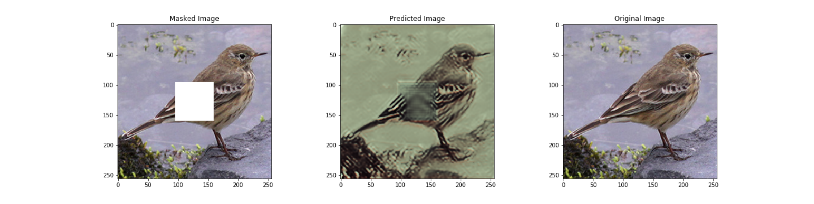
\includegraphics[width=80mm, keepaspectratio]{figures/err_1.png}
\end{figure}

\begin{figure}[H]
  \centering
  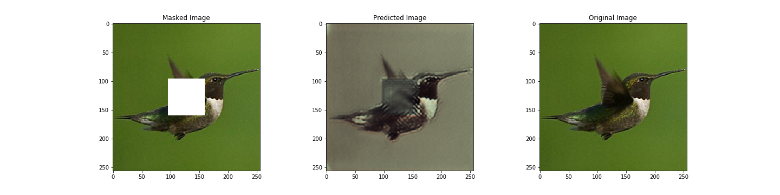
\includegraphics[width=80mm, keepaspectratio]{figures/err_2.png}
\end{figure}

\begin{figure}[H]
  \centering
  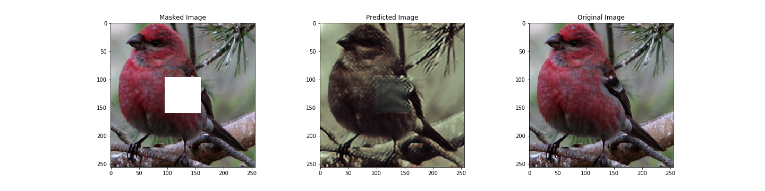
\includegraphics[width=80mm, keepaspectratio]{figures/err_3.png}
\end{figure}

These pictures are the results of previous trainings 
The old solution to the mentioned problem was post-processing, which was a computationally expensive process, as well as an unreliable one, as it often failed.
Partial convolutions are a relatively newly introduced solution to the image inpainting problem 

\section{Data acquisition and preparation}
We used the Caltech-UCSD Birds-200-2011 dataset \cite{dataset}. It consists of 11788 annotated photos of 200 different bird species.

As preparation, we calculated the minimal bounding square of birds according to their bounding boxes. Through this process, we threw away the images where the bounding box couldn't be contained in a square due to the original image dimensions. We then scaled the resulting square to a resolution of 256  $\times$ 256 pixels.

This way we got 9581 images which we splitted into train, validation and test sets in a 6:2:2 ratio. 

For the training, we use a 64 $\times$ 64 pixel hole in the center of the image.

\begin{figure}[H]
  \centering
  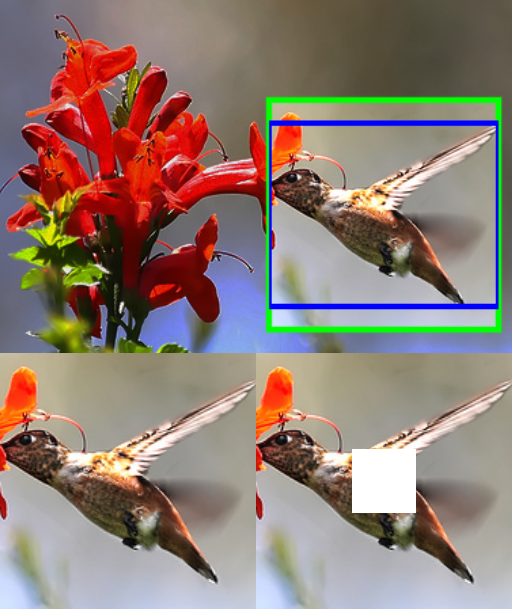
\includegraphics[width=80mm, keepaspectratio]{figures/preparation.png}
  \caption{The original image with bounding box (blue) and the minimal square (green) and the resulting image with the applied mask}
  \label{fig:Preparation}
\end{figure}


\section{Training the network}

Training the network happens in two main stages. The first one is the initial stage, where the network’s weights are initialized with the weights of the VGG16 model. In this stage we used a learning rate of 0.0002 with batch normalization on. We run this for 60-70 epochs. In each epoch we have 1000 training and 1000 validation steps. At the end of each epoch we save the model checkpoint. After that comes the fine tuning of the model, where we load the weights from the latest saved checkpoint. This runs for about 50 epochs with a learning rate of 0.00005. The batchsize is 6 in every stage of the training. (however we were able to keep this batch size only in the cloud, the GTX 1060 throws a memory exhaustion error with batch sizes greater than 2) One epoch takes about 3 minutes of training and 3 minutes of validation with 1000-1000 images each. To achieve usable results we had to train the network for about 7 hours with the weights loaded from VGG 16 in stage 1, and another 7 hours of fine tuning was needed in stage 2. Because the training takes so long we didn't have too much room for experimenting, and the slightest change from the recommended hyperparameters ended up in totally useless results. Even so we tried to play with the learning rate by adding two more stages to the training with learning rates of 0.00015 and 0.0001, but that didn't improve the quality of the solution. It was interestnig, that in the second stage, where we had to turn off batch normalization by recommendation, we got better results by leaving it on. We also did some experiments for speeding up training by decreasing the validation steps from 1000 to 100. This way one epoch takes about 4 minutes with validation included, so it's spares about 30-40\% of the training time, and the results are still acceptable. Maybe it's worth mentioning that when training on the local machine the GPU ran only at 20\% load, but we couldn't figure out the reason. The training data is split into train, validation and test folders. The datagenerators used during the training are AugmentingDataGenerator instances. There are three of them: one for training, one for valitation,and one for testing. These generators will get a picture from the appropriate folder and apply a centered 64 $\times$ 64 sized square shaped mask on it.

\begin{figure}[H]
  \centering
  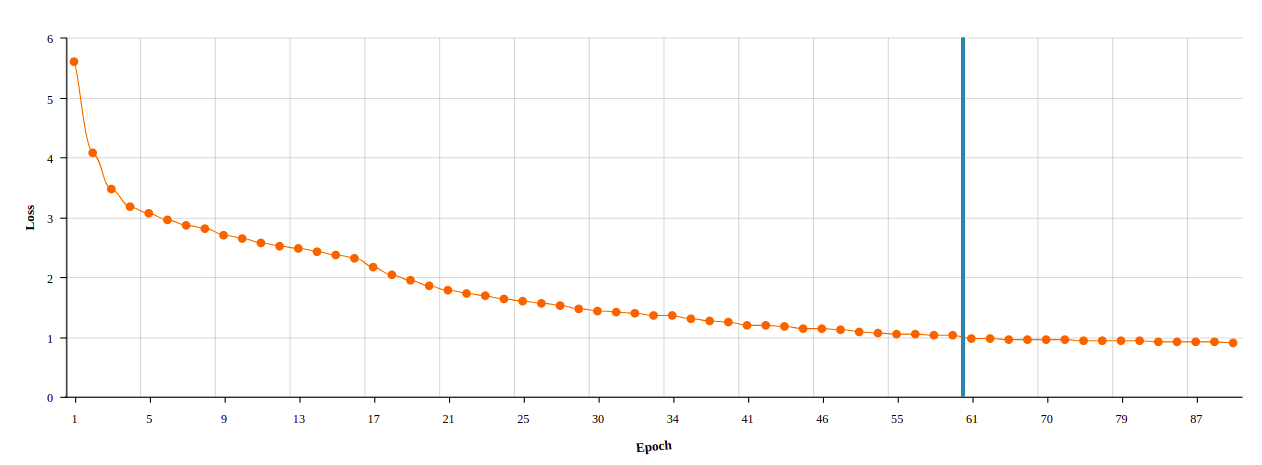
\includegraphics[width=80mm, keepaspectratio]{figures/loss_change.png}
  \caption{The change of loss through the training process. The blue line denotes the point where we changed the applied learning rate}
\end{figure}
\pagebreak
\section{Results}

\begin{figure}[H]
  \centering
  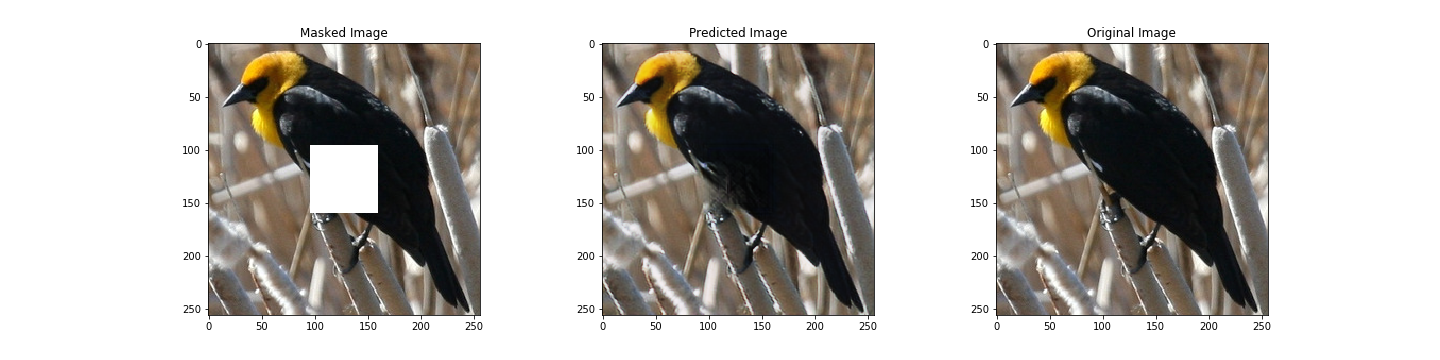
\includegraphics[width=80mm, keepaspectratio]{figures/result_1.png}
\end{figure}

\begin{figure}[H]
  \centering
  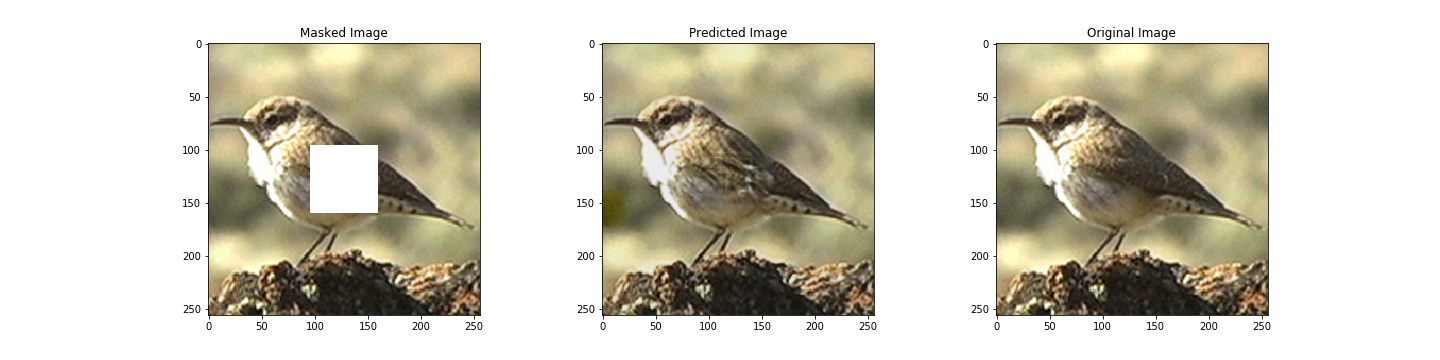
\includegraphics[width=80mm, keepaspectratio]{figures/result_2.png}
\end{figure}

\begin{figure}[H]
  \centering
  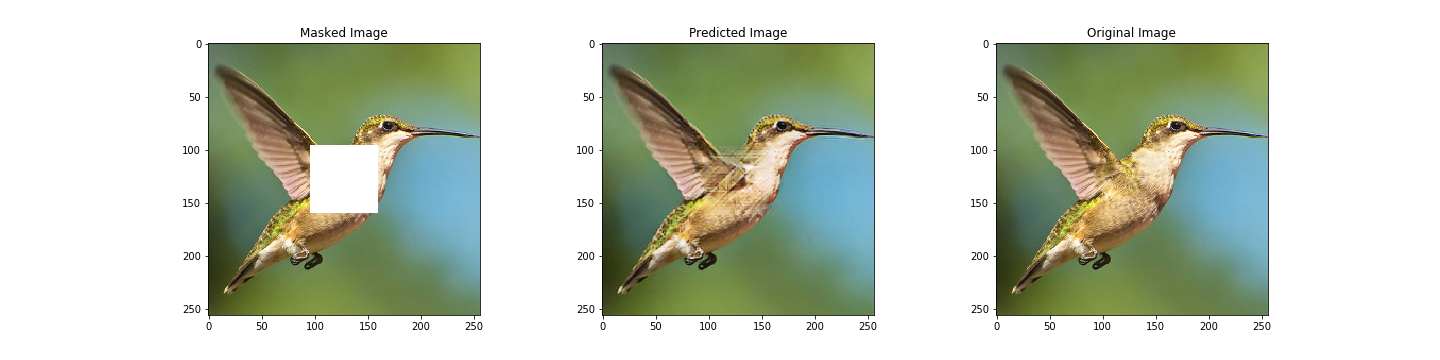
\includegraphics[width=80mm, keepaspectratio]{figures/result_3.png}
\end{figure}

\begin{figure}[H]
  \centering
  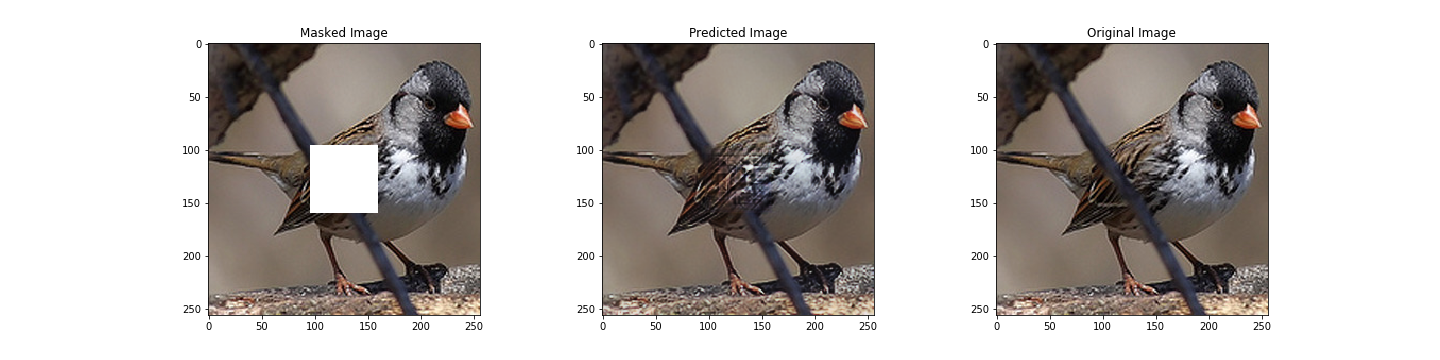
\includegraphics[width=80mm, keepaspectratio]{figures/result_4.png}
\end{figure}

\begin{figure}[H]
  \centering
  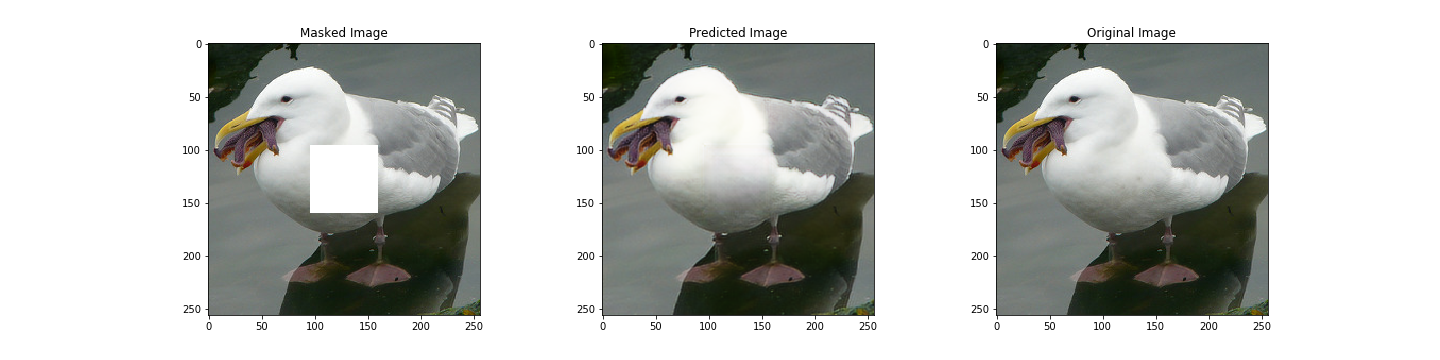
\includegraphics[width=80mm, keepaspectratio]{figures/result_5.png}
\end{figure}

As you can see in the pictures, the results are mixed. Generally speaking, the network was able to fill out the pictures, and it added relevant details, completed feather patterns and limbs. However, in unusual situations, such as fast moving birds or birds with part of them hidden behind objects, the network was unable to correctly guess the original image. 
The reason behind this is most likely due to the scarce nature of such photographs in the training database. Which is to be expected. 
However, all things considered the results are more than acceptable, and exceeded our expectations in situations where the feather pattern was recognisable, and in a few places even in difficult situations. (e.g: the 2nd picture, where the lighting is really difficult, and the feather pattern is mostly hidden as well.)

\section{Summary}

In our first approach we only tried to train the network in a narrow domain (bird pictures), and with a centered, square shaped mask. At the end of the work we have made another quick training on another dataset (16000 car pictures) with similar results. Next we woluld like to try training it with irregular masks suggested by Liu \cite{nvidia_paper}, and try to utilize the capabilities of the network for image superresolution upsampling by ofsetting the pixels of the image and using the missing pixels as an irregular mask. Another experiment could be trying it with a different pretrained networks for feature extraction, or training the network on multiple domains at once, and comparing the results with the approaches where we only used a single domain as a training dataset.

\vspace{20px}
\begin{thebibliography}{00}

\bibitem{dataset} Wah, C. and Branson, S. and Welinder, P. and Perona, P. and Belongie, S., ``The Caltech-UCSD Birds-200-2011 Dataset'', California Institute of Technology, CNS-TR-2011-001, 2011

\bibitem{nvidia_paper} Guilin Liu, Fitsum A. Reda, Kevin J. Shih, Ting-Chun Wang, Andrew Tao, Bryan Catanzaro, ``Image Inpainting for Irregular Holes Using Partial Convolutions'', arXiv:1804.07723v2  

\bibitem{pconv_keras} https://github.com/MathiasGruber/PConv-Keras/

\bibitem{} Bertalmio, M., Sapiro, G., Caselles, V., Ballester, C., ``Image inpainting. In: Proceedings of the 27th annual conference on Computer graphics and interactive techniques'', pp. 417–424. ACM Press/Addison-Wesley Publishing Co. (2000)  

\bibitem{} Jiahui Yu, Zhe Lin, Jimei Yang, Xiaohui Shen, Xin Lu, Thomas S. Huang, ``Generative Image Inpainting With Contextual Attention. In: IEEE Conference on Computer Vision and Pattern Recognition (CVPR)'', pp. 5505-5514, 2018

\bibitem{} Dai, J., Qi, H., Xiong, Y., Li, Y., Zhang, G., Hu, H., Wei, Y., ``Deformable convolutional networks'', CoRR, abs/1703.06211 1(2), 3, 2017

\bibitem{} Harley, A.W., Derpanis, K.G., Kokkinos, I., ``Segmentation-aware convolutional networks using local attention masks'', In: IEEE International Conference on Computer Vision (ICCV). vol. 2, p. 7, 2017

\bibitem{} He, K., Zhang, X., Ren, S., Sun, J., ``Delving deep into rectifiers: Surpassing humanlevel performance on imagenet classification'', In: Proceedings of the IEEE international conference on computer vision. pp. 1026–1034, 2015

\end{thebibliography}

\end{document}